\documentclass{article}

% Language setting
% Replace `english' with e.g. `spanish' to change the document language
\usepackage[italian]{babel}
\usepackage{float}
\usepackage{subfig}

% Set page size and margins
% Replace `letterpaper' with `a4paper' for UK/EU standard size
\usepackage[letterpaper,top=2cm,bottom=2cm,left=3cm,right=3cm,marginparwidth=1.75cm]{geometry}

% Useful packages
\usepackage{amsmath}
\usepackage{graphicx}
\usepackage{float}
\usepackage[colorlinks=true, allcolors=blue]{hyperref}

\setlength{\parskip}{6pt}%

\title{Simulatore del movimento dei pianeti in un sistema solare}
\author{Gioele Mancino, Federico Mastroforti, Luca Tesei, Nico Tortorici}

\begin{document}
\maketitle
\section{Il Progetto}
\subsection{Istruzioni per la compilazione}
All'interno del compilatore è necessario scaricare la repository online utile per la creazione della GUI:
\begin{verbatim}
   $ sudo add-apt-repository ppa:texus/tgui
   $ sudo apt-get update
   $ sudo apt-get install libtgui-1.0-dev
    \end{verbatim}
Poi possiamo compilare tramite CMake usando questi comandi:
\begin{verbatim}
    $ cmake -S. -B build
    $ cmake --build build
    $ build/gravity
     \end{verbatim}

\subsection{Obiettivo del simulatore}
Si vuole creare un programma in grado di calcolare in tempo reale e rappresentare tramite
un'interfaccia il movimento di alcuni corpi celesti e le interazioni tra loro. è inoltre possibile aggiungere nuovi pianeti direttamente all'interno della simulazione che interagiranno con quelli già presenti.

\subsection{Interface}
\subsubsection{Elements on screen}
Nell'angolo in alto a sinistra (Figura \href{playpause} ) troviamo 2 pulsanti cliccabili (che vedremo nel dettaglio nella prossima sezione), 
il tempo trascorso dall'inizio della simulazione (in anni, espresso con 7 cifre significative) e la velocità espressa in rapporto di tempo (anni al secondo)

\subsubsection{User interaction}
Nell'angolo alto a sinistra dell'interfaccia grafica sono presenti due tasti: \\
-il tasto Play/Pause (Figura \href{playpause}, sinistra ) che permette di far partire o fermare la simulazione;\\
-il tasto Reset (Figura \href{playpause}, destra) che riporta tutto allo stato iniziale (i corpi già presenti ritornano nel punto in cui erano a inizio simulazione mentre quelli generati dall'utente vengono eliminati); \\
In tutta la finestra grafica è possibile cliccare con il tasto destro in un punto, facendo ciò comparirà una finestra in cui è possibile inserire la massa del corpo che stiamo inserendo (in unità di massa terrestre) e sarà poi possibile selezionare il verso di movimento iniziale del corpo

\begin{figure} [H]
    \centering
    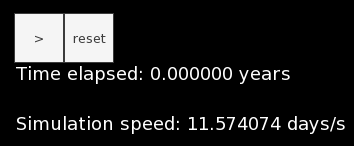
\includegraphics[height=.20\linewidth]{Playpause.png}
    \captionof{figure}{Il tasto (sinistra) Play/Pause permette di far partire e fermare la simulazione in ogni momento, mentre il tasto (destra) reset riporta la simulazione allo stato iniziale  (i corpi già presenti ritornano nel punto in cui erano a inizio simulazione mentre quelli generati dall’utente vengono eliminati) }
    \label{playpause}
\end{figure}

\subsection{La fisica dietro al programma}
La legge di gravitazione universale afferma che due punti materiali si attraggono con una forza di intensità direttamente proporzionale al prodotto delle masse dei singoli corpi e inversamente proporzionale al quadrato della loro distanza. Questa legge, espressa vettorialmente, diventa:
\begin{equation}
\textbf{F}_{2,1}(\textbf{r})=-\frac{Gm_{1}m_{2}}{r^{2}}\textbf{u}_{r}
\end{equation}
dove $\textbf{F}_{2,1}$ è la forza con cui l'oggetto 1 è attratto dall'oggetto 2, G è la costante di gravitazione universale, che vale circa $6,67\cdot 10^{-11}\frac{Nm^2}{kg^2}$, $m_1$ e $m_2$ sono le masse dei due corpi, $\textbf{r}=\textbf{r}_1-\textbf{r}_2$ è il vettore congiungente i due corpi (supposti puntiformi), 
$r$ è il suo modulo e $\textbf{u}_r=\frac{\textbf{r}}{r}$ rappresenta il versore che individua la retta congiungente i due punti materiali.\\
Il programma utilizza questa relazione per calcolare istante per istante le forze che agiscono su ogni corpo, e di conseguenza le accelerazioni:
\begin{equation}
\textbf{F}_{j,tot}=\sum_{i=1, i≠j}^{N_{bodies}}\textbf{F}_{i}(\textbf{r})=m\ddot{\textbf{r}}
\end{equation}
dove \textbf{F}_{j,tot} è la forza risultante che agisce sul corpo $j$.\\
Integrando poi la precedente equazione si ottiene la legge oraria $\textbf{r}(t)$ del corpo $j$. Non essendo risolvibile analiticamente si deve ricorrere a metodi di integrazione numerica.


\section{Strumenti di sviluppo}
\subsection{C++}
\subsection{Librerie esterne}
\subsection{CMake}
\subsection{VSCode}
\subsection{Git e Github}
\section{Implementazione}
\subsection{Metodo Leapfrog}
\subsection{Struttura del progetto}
\section{Testing e debugging}
\section{Risultati e problemi riscontrati}
\appendix
\section{Calcoli e approssimazioni}

\end{document}